\newpage
\part{Détection du tag}

La détection du tag est une partie crutiale de cette application de réalité augmentée. L'objectif est de récupérer les coordonnées du tag dans la caméra pour avoir les informations sur l'orientation et la distance de la scène à projeter sur l'image.

    \section{Détection complète}

    Dans les grandes lignes, la détection du tag consiste à récupérer toutes les formes qui pourraient correspondre au tag dans l'image, puis de trouver la forme qui correspond au véritable tag que nous cherchons. L'orientation et la distance du tag détecté servira ensuite pour projeter les objets dans la scène.

    Une fois le tag détecté, l'application tentera de le tracker lors des images suivantes de la vidéo, afin de gagner en temps de calcul en évitant de refaire tout le processus. Si le tracking ne parvient pas à suivre le tag (mouvement trop important de la caméra par exemple), une nouvelle détection complète est effectuée.

        \subsection{Modèle de tag}

        Le tag consiste à une grille en deux dimensions qui représente un code binaire matérialisé par des cases noires ou blanches.

        \begin{figure}[!h]
            \centering
            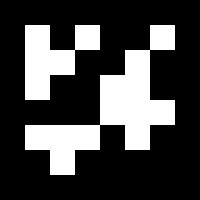
\includegraphics[scale=0.25]{img/marker.jpeg}
            \caption{Tag à détecter}
        \end{figure}

        Dans l'application, le tag est décomposé dans un tableau de 64 éléments qui comporte ces 0 ou ces 1.

        Ce tableau est créé au lancement de l'application, avec l'image du tag passé en paramètre.

        Le même processus est réalisé pour un tag qui sera détecté dans l'image. Son code sera lu puis découpé dans un tableau de 64 éléments et les deux tableaux seront comparés et déterminer si le contenu des deux codes correspond.  

        \subsection{Extraction des tags potentiels}

        La première étape consiste à sortir de l'image les quadrilatères qui peuvent potentiellement correspondre à des tags.

        Pour cela, un prétraitement est d'abord effectué sur l'image. L'image est convertie en niveau de gris puis binarisée à l'aide d'un seuillage adaptatif (une valeur de seuil sera determinée en fonction des régions, qui peut différer donc d'une région à l'autre).

        \begin{figure}[!h]
            \centering
            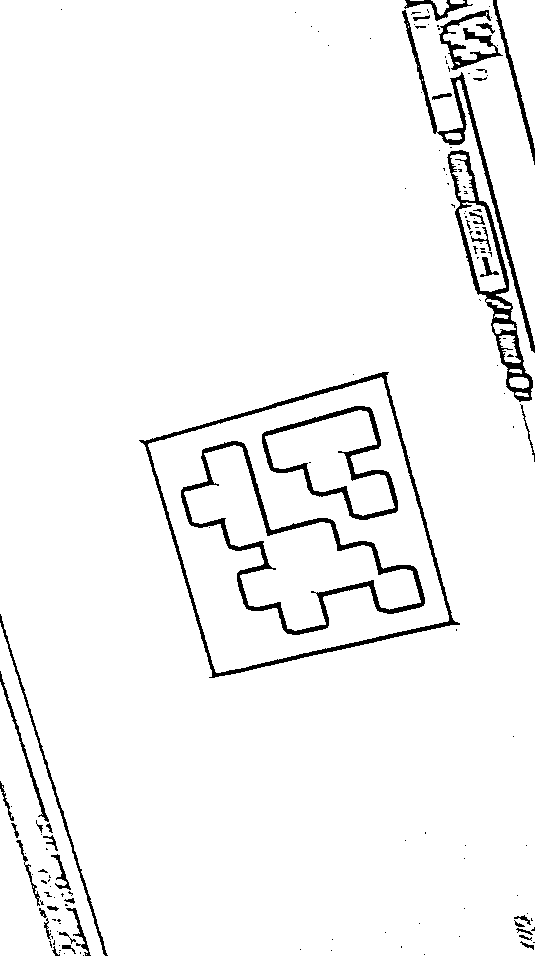
\includegraphics[scale=0.25]{img/threshold.png}
            \caption{Image seuillée}
        \end{figure}

        Une fois l'image binarisée, nous pouvons effectuer une détection de contours sur cette dernière.

        La méthode \textit{findContours}, que nous utilisons fournie par OpenCV, renvoie pour chaque contour détecté une liste de points. Nous souhaitons à partir de ces points créer une forme qui va recouvrir le contour. Pour cela, nous allons générer une enveloppe convexe pour ces points.

        C'est à dire que nous allons englober de manière la plus optimale possible tous les points communs à un contour dans une forme convexe.

        \begin{figure}[!h]
            \centering
            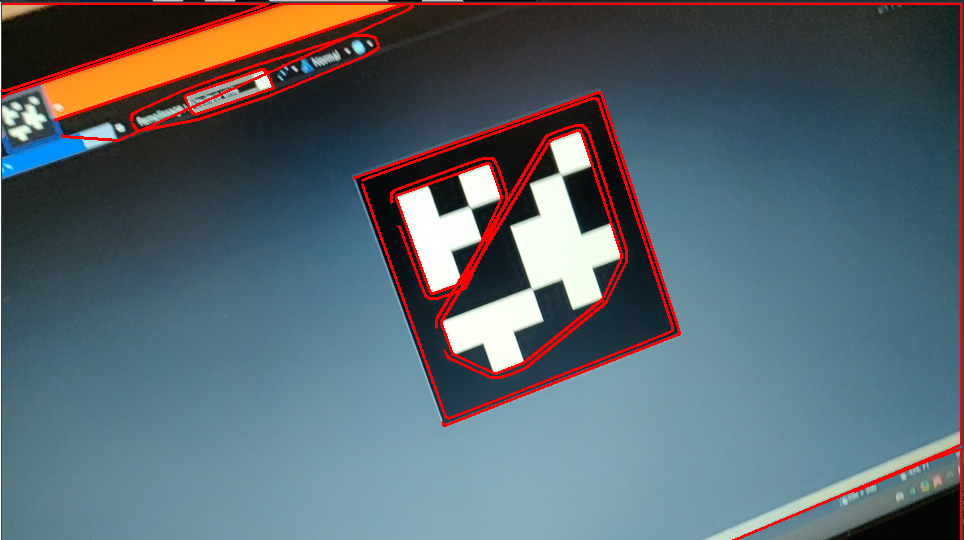
\includegraphics[scale=0.25]{img/convex_hull.png}
            \caption{Chaque contour de l'image est englobé}
        \end{figure}

        Certains contours détectés peuvent être formés de manière complexe (enchaînements de points pour au final un polygone avec un petit nombre de côtés) et risquerons de fausser la détection de contours quadrilatères. Pour gérer cela, nous ajoutons une étape où les points proches entre eux ou alignés sur un contour sont supprimés.

        EXPLIQUER ?

        Avec ces contours désormais nettoyés, nous pouvons récupérer tous les contours de forme quadrilatère, qui correspondent à tous les candidats pour être le tag que nous recherchons.

        \subsection{Identification du tag correct}

        Tous les tags candidats sont ensuite comparés au modèle de tag que nous voulons reconnaître.

        \subsubsection{Homographie}

        Le candidat sur l'image est déformé par rapport au modèle de tag qui sera nécessaire afin de comparer les deux images.

        Une première étape est en conséquence nécessaire pour redresser cette image afin qu'elle soit de la même taille et forme que l'image à comparer.

        Nous allons pour ceci estimer l'homographie entre l'image avec le candidat déformé et un carré parfait, la forme qui est visée et qui correspond au modèle de tag que nous possédons.

        \begin{figure}[h]
            \centering
            \subfloat[][Tag candidat déformé]{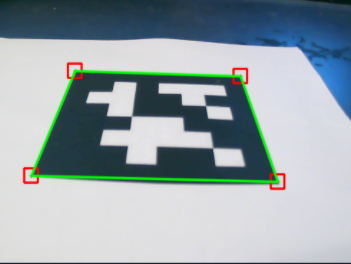
\includegraphics[width=0.48\linewidth]{img/beforewrap.png}}
            \hspace{.02\textwidth}
            \subfloat[][Forme visée]{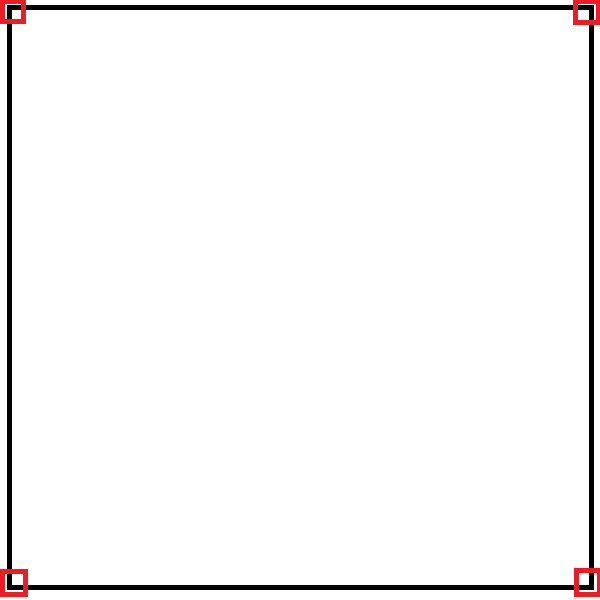
\includegraphics[width=0.38\linewidth]{img/tag_homography_target.png}}
            \caption{On cherche a estimer l'homographie entre ces deux représentations du tag candidat pour le redresser}
        \end{figure}

        L'estimation de l'homographie est en effet une transformation entre deux plans qui nous permettera de stocker dans une matrice d'homographie les informations relatives notamment à la rotation et translation entre ces deux plans.

        \textbf{\textit{Estimation de la matrice d'homographie}}

        Bien qu'OpenCV dispose de méthodes pour estimer une matrice d'homographie entre deux jeux de points, nous avons décidé de réimplémenter une solution d'estimation d'homographie.

        Comme vu précédemment, on cherche à établir la transformation entre deux images. C'est à dire, pour chaque couple de points $p_i \leftrightarrow p_{i}' $, nous cherchons la matrice $H$ telle que :
    
        \begin{center}
            $ p_i = Hp_i' $            
        \end{center}

        Avec :

        \begin{itemize}
            \item $ p_i $ correspondant aux points de départ, ou ici de l'image déformée.
            \item $ p'_i $ correspondant aux points d'arrivés, ou ici d'un cadre droit, la forme visée.
        \end{itemize}
            
        Nous pouvons développer donc pour tout point $p_i$ :
    
        \[
            \begin{pmatrix}
                x_i \\
                y_i \\
                1      
            \end{pmatrix}
            = 
            \begin{pmatrix}
                h1 & h2 & h3 \\
                h4 & h5 & h6 \\
                h7 & h8 & h9      
            \end{pmatrix} 
            \times
            \begin{pmatrix}
                x'_i \\
                y'_i \\
                1      
            \end{pmatrix}
            \]
        
        L'objectif est donc de déterminer la matrice H telle que :
    
        \begin{center}
        $ H = \begin{pmatrix} h1 & h2 & h3 \\ h4 & h5 & h6 \\ h7 & h8 & h9 \end{pmatrix} $
        \end{center}
    
        On peut réécrire l'estimation de l'homographie dans un premier temps pour un point de cette manière :

        \begin{center}
            $x_i = \frac{h1x'_i + h2y'_i + h3}{h7x'_i + h8y'_i + h9} $  
        \end{center}
    
        \begin{center}
            $y_i = \frac{h4x'_i + h5y'_i + h6}{h7x'_i + h8y'_i + h9} $
        \end{center}
    
        Qui est égal à :
    
        \begin{center}
            $ x'_ih1 + y'_ih2 + h3 - x'_i x_ih7 - y'_ix_ih8 - x_ih9 = 0 $
    
            $ x'_ih4 + y'_ih5 + h6 - x'_iy_ih7 - y'_iy_ih8 - y_ih9 = 0 $
        \end{center}

        Nous nous retrouvons sous la forme d'un système de 2 équations à 9 inconnues.

        On observe du coup qu'un couple de point mène donc à deux équations qui permettent de résoudre $H$.
    
        Nous pouvons d'ailleurs par avance résoudre h9, car dans le cas d'une homographie, nous avons toujours $h9 = 1$.
    
        Il nous reste huit inconnues à résoudre : 4 points sont alors nécessaires pour générer 8 équations dans le système, dont on considère $h9$ comme déjà résolu : 

        \[
        \begin{pmatrix} 
            x_1 & y_1 & 1 & 0 & 0 & 0 & -x_1 x'_1 & -y_1 x'_1 \\ 
            0 & 0 & 0 & x_1 & y_1 & 1 & -x_1 y'_1 & -y_1 y'_1 \\
    
            x_2 & y_2 & 1 & 0 & 0 & 0 & -x_2 x'_2 & -y_2 x'_2 \\ 
            0 & 0 & 0 & x_2 & y_2 & 1 & -x_2 y'_2 & -y_2 y'_2 \\
    
            x_3 & y_3 & 1 & 0 & 0 & 0 & -x_3 x'_3 & -y_3 x'_3 \\ 
            0 & 0 & 0 & x_3 & y_3 & 1 & -x_3 y'_3 & -y_3 y'_3 \\
    
            x_4 & y_4 & 1 & 0 & 0 & 0 & -x_4 x'_4 & -y_4 x'_4 \\ 
            0 & 0 & 0 & x_4 & y_4 & 1 & -x_4 y'_4 & -y_4 y'_4
        \end{pmatrix} 
        \times
        \begin{pmatrix} h1 \\ h2 \\ h3 \\ h4 \\ h5 \\h6 \\ h7 \\ h8 \end{pmatrix}
        =
        \begin{pmatrix} x'_1 \\ y'_1 \\ x'_2 \\ y'_2 \\ x'_3 \\ y'_3 \\ x'_4 \\ y'_4 \end{pmatrix} 
        \]
    
        Nous disposons de ces couples de points dans notre cas car nous avons déjà détecté d'une part les coins du tag candidat que l'on cherche à redresser, et d'autre part nous connaissons déjà les coordonnées des points d'arrivée, sous la forme d'un carré. Nous pouvons donc créer ce système d'équation à partir de ces quatre couples de points.

        Un pivot de Gauss est réalisé sur ce système d'équations. Une fois ce pivot résolu, nous obtenons une matrice en "row echelon form", c'est à dire :
    
        \begin{itemize}
            \item Toutes les lignes qui ne sont pas entièrement constituées de 0 commencent par un 1
            \item Pour deux lignes non constituées que de 0, la valeur 1 de la ligne placée en haut de la matrice sera plus à gauche que le 1 de la ligne placée plus bas
            \item Toutes les lignes avec seulement des 0 sont placées en bas
        \end{itemize}
    
        Nous effectuons en conséquence une "back substitution" pour faire apparaître la solution sur la dernière colonne.
    
        La dernière colonne du système est donc la résolution de la matrice $H$, qui nous donne notre matrice d'homographie.

        Cette méthode permet d'estimer de manière fiable la matrice d'homographie entre l'image avec le candidat et une image droite.

        
            \subsubsection{Wrap Perspective}

            Maintenant que la matrice d'homographie est établie, nous devons l'utiliser pour redresser l'image deformée dans la forme souhaitée.

            ... 

            Cependant, dans le cas où la caméra aie prise l'image à l'envers, le tag candidat sera inversé par rapport au modèle à comparer. Le candidat, bien que valide, ne serait donc pas détecté. Pour contrer cela, nous allons par quatre fois effectuer une rotation sur l'ordre des points du contours pour tester toutes les orientations possibles.


        \begin{figure}[h]
            \centering
            \subfloat[][Image originale]{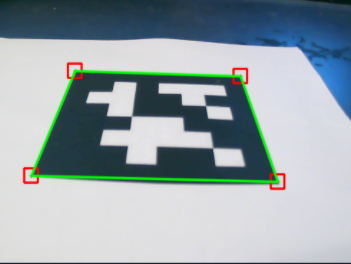
\includegraphics[width=0.48\linewidth]{img/beforewrap.png}}
            \hspace{.02\textwidth}
            \subfloat[][Tag potentiel extrait]{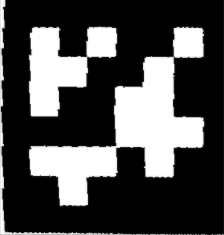
\includegraphics[width=0.35\linewidth]{img/afterwrap.png}}
            \caption{Wrap Perspective sur la première image pour recadrer le tag potentiel}
        \end{figure}
            

        \subsection{Résumé de la procédure}

        Pour résumer, la détection du tag consiste à :

        \begin{itemize}
            \item Réaliser un seuillage adaptatif sur l'image
            \item Réaliser un convex hull sur les contours
            \item Nettoyer les contours
            \item Estimer l'homographie
            \item Effectuer la Wrap Perspective
            \item Comparer au modèle de tag
        \end{itemize}

    \subsection{Tracking}

    
    \section{Amélioration de la détection du tag}

    Après les premiers tests, nous avons remarqué que la détection du tag était efficiente lorsque le tag était bien visible quel que soit sa rotation ou sa taille, mais perdait en efficacité lors de mouvements plus brusques de la caméra, notamment à cause du flou de mouvement.

    Nous avons implémenté deux méthodes pour rendre plus robuste cette détection afin de détecter le tag même lors des mouvements de la caméra.

        \subsection{Défloutage gaussien}

        Une première méthode pour optimiser la détection du tag est de retirer le bruit causé par le flou de mouvement de la caméra lorsque le tag n'est pas détecté.

        Pour cela, on va considérer que le flou est causé par un flou gaussien. L'objectif est de soustraire l'image floutée par sa propre image non floutée.

        Nous appliquons un flou gaussien sur l'image bruitée. Ensuite, nous calculons la somme pondérée de l'image d'entrée et l'image floutée, avec un poids de $1.5$ pour l'image d'entrée et un poids de $-0.5$ pour l'image floutée. Nous prenons en réalité l'image bruitée par le flou de mouvement, auquel nous soustrayons l'image floutée par le filtre gaussien. Ceci permet d'éliminer une partie du flou sur l'image original et d'affiner les contours.

        \subsection{Marge d'acceptation de détection du tag}

        Comme nous l'avons vu précédemment, chaque tag potentiel détecté sur l'image est comparé au modèle de tag pour vérifier si les 64 cases du candidat correspondent bien au tag que nous cherchons.

        Lors du mouvement de la caméra, il peut arriver que le flou de mouvement empiète sur certaines cases et modifie légèrement le résultat, ce qui en conséquence écarte le tag de la recherche.

        Nous pouvons en conséquence tolérer un seuil d'acceptation du tag, où si jamais entre 5 et 10 \% des cases du potentiel tag ne corrèlent pas au modèle, le candidat est quand même accepté comme étant le tag, car si observons une correspondance par exemple sur 56 cases du tag sur les 64, nous pouvons être quasiment sûr qu'il s'agit bien du tag que nous recherchons.

        \subsection{Résultats}

        Les deux méthodes indépendamment améliorent, mais pas de façon considérable, les résultats, mais en les combinant nous parvenons à avoir une détection plus robuste.

        \begin{figure}[!h]
            \begin{center}
                \begin{tabular}{ | c | c | c | c | c | }
                \hline
                Vidéo & Sans optimisation & Approximation & Défloutage Gaussien & Combinaison \\ \hline
                Vidéo 1 & 88.2\% & 91.4\% & 90.9\% & 94.1\% \\ \hline
                Vidéo 2 & 12.21\% & Non testé & Non testé & 37.40\% \\
                \hline
                \end{tabular}
        \end{center}
        \caption{Taux de détection du tag par vidéo}
        \end{figure}

        Vidéo 1 : Vidéo de plutôt bonne qualité, le tag sort de l'écran une seconde

        Vidéo 2 : Vidéo de mauvaise qualité, plus de mouvement de la caméra, le tag est plus petit et légèrement froissé.

        Bien que la détection avec ces méthodes reste généralement de bonne qualité, il y a malgré tout plus de risque d'avoir une détection d'être dégradée, comme il peut être observé sur l'image ci-dessous.

        \begin{figure}[!h]
            \centering
            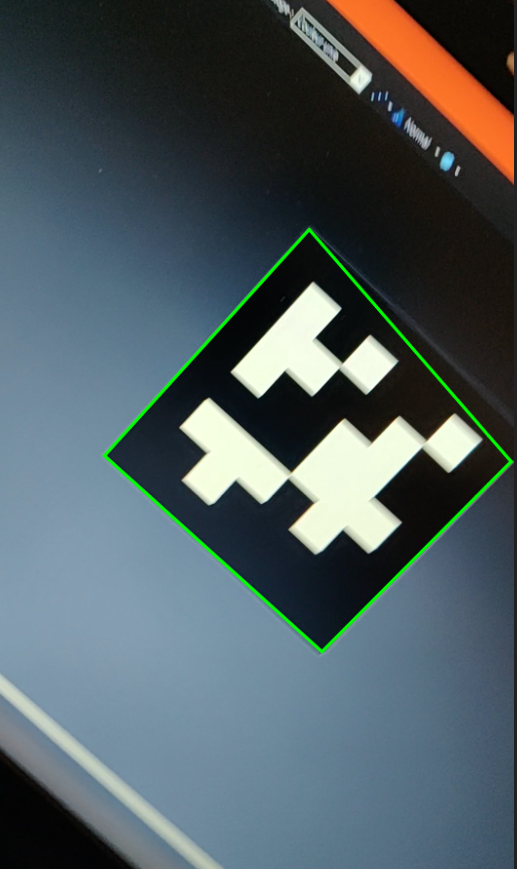
\includegraphics[scale=0.25]{img/cropped_tag.png}
            \caption{Le tag est détecté, mais un angle n'est pas bien géré}
        \end{figure}

        Pour éviter de dégrader la détection des contours lors des frames suivantes du flux vidéo, nous ne réalisons pas de tracking sur le tag que nous avons détecté à l'aide des méthodes d'optimisations, car il sera éventuellement possible de trouver un tag parfait lors de la frame suivante, qui serait de meilleur qualité qu'un tag de moins bonne qualité tracké par rapport à celui de la frame précédante.

        Cette petite marge d'erreur permet entre autre également de gérer partiellement l'occlusion du tag. En effet, un obstacle de petite taille cachant seulement quelques cases du tag peut ne pas poser de problème à sa détection, étant donné que les autres cases du tag seraient tout de même détectées.

        IMAGE OCCULSION TAG ? 

        De plus, ces méthodes d'optimisations ne permettent pas de détecter le tag lorsqu'il sort de l'écran.